\begin{section}{Molecular Simulation: Cost Considerations}

Calculations of a \pes ultimately rely on finding approximate solutions to
the time-independent Schr\"odinger equation,
\begin{align}
\label{eq:intro-se}
\hat{H}\Psi = E\Psi
\end{align}
where $\hat{H}$ is a quantum-mechanical operator describing both the kinetic
and potential energies of the nuclei and electrons, $\Psi$ is a wavefunction,
and $E$ is the energy of the system as a function of the nuclear coordinates. A plethora of
approximations exist for solving \cref{eq:intro-se}, each with their own
disadvantages and advantages, and a full discussion of the accuracy of such
\glspl{est} can be found in \citet{Cramer2004} and other texts.
These methods differ greatly into terms of
computational cost with respect to system size, and so we begin our
discussion of \glspl{est} in terms of the cost-efficiency with which various
methods might be used in molecular simulation.
%
At the high cost end of the spectrum, extremely accurate `gold-standard' \est
calculations can be run using a method known as
\ccsdt, whose cost scales as $N^7$
with respect to the number of electrons in the system. More approximate
methods, such as
MP2 and HF, scale as $N^5$ and $N^4$, respectively, and \dft (frequenctly regarded
as the 
`computationally-affordable' workhorse of \est) scales even more modestly as $N^3$.
To put these scalings in context,
however,
\cref{fig:intro-scaling} shows the largest system sizes (given as a number of
atoms) which a given \est is capable of computing using available
computational resources. 
Though these estimates are taken from the early 2000s (since which
the `TeraFlops MPP' supercomputer has been superseded in 2016 by
various PetaFlops supercomputers with 1000x the computer power), several of
the conclusions are still the same, namely that \ccsdt and most other
\glspl{est} remain too expensive to be employed in large-scale molecular
simulation.

%%%%%%%%%%%%%%%%%%%% Scaling and Computer Power %%%%%%%%%%%%%%%%%%%%%%%%%%%
\begin{figure}
\centering
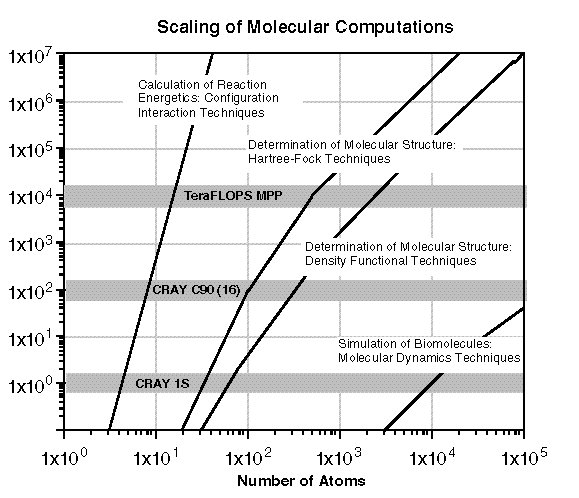
\includegraphics[width=\textwidth]{intro/scale.png}
\caption{
The relative computing power required for molecular computations at four
levels of theory. In the absence of screening techniques, the formal scaling
for configuration interaction, Hartree-Fock, density functional, and molecular
dynamics is: N6, N4 , N3 and N2 , respectively.
Reprinted from \citen{Guest2001} with permission.
    }
\label{fig:intro-scaling}
\end{figure}
%%%%%%%%%%%%%%%%%%%% Scaling and Computer Power %%%%%%%%%%%%%%%%%%%%%%%%%%%

Compounding the above scaling problem, molecular simulation requires that we
compute,
not just one snapshot of a molecular \pes, but millions, billions, or 
(for protein folding simulations) even trillions of such energy snapshots.
Thus depending on the lengths and timescales
involved in the chemical processes under study, even the cheapest \dft \glspl{est}
are typically too expensive for routine molecular simulation.
(For reference, in 2014 \dft-based simulations were reported on 
roughly $10^3$-atom systems using state-of-the-art facilities,
\cite{Ballone2014}
whereas $10^5-10^6$ atoms can be required for running representative
simulations of proteins.\cite{Karplus2002,Lane2013})

As computing power continues to increase, there is no doubt that advanced and
accurate \glspl{est} will eventually be used in larger-scale molecular
simulation to investigate problems of both chemical and biological
import.\cite{Ballone2014} In
the meantime, however, and for investigating problems on extremely large time-
and length-scales, lower-cost methods for calculating the \pes are required.
In order to achieve this low-cost scaling, a popular strategy is to model the
\pes using simple mathematical expressions which depend only on the positions
of the nuclei in the system. Such models are referred to as `force fields',
which are defined both by the choice of functional forms (that is,
mathematical formulae) and parameters that go into them.
The computational cost of force fields nominally scales as $N^2$ (and usually
scales as $N\log N$ in
practice) with respect
to the number of \emph{atoms} (rather than electrons) in the system, thus
representing significnat computational savings compared to
the \glspl{est} described above.
\cref{fig:intro-scaling} shows the scaling of these methods in the $N^2$
scaling limit, from which it becomes clear that we can use force fields
to study system sizes 2--3 \emph{orders of magnitude} larger than what is
possible with \dft.
%
Indeed, in the early 1990s \citet{Chan1993} provided a useful estimation
of the computing power needed to simulate a variety of 
important chemical and biological processes (\cref{fig:intro-timeline}), and showed that,
using these cost-efficient force fields,
we are not far off from the time when atomistic simulations of protein folding and/or aggregation
can be achieved.
Some of the first simulations of protein
folding have already been reported, and using computationally-efficient force
fields we can expect this trend to continue
into the foreseeable future.\cite{Lane2013}


%%%%%%%%%%%%%%%%%%%% Simulation Timeline %%%%%%%%%%%%%%%%%%%%%%%%%%%%%%%%%%%
\begin{figure}
\centering
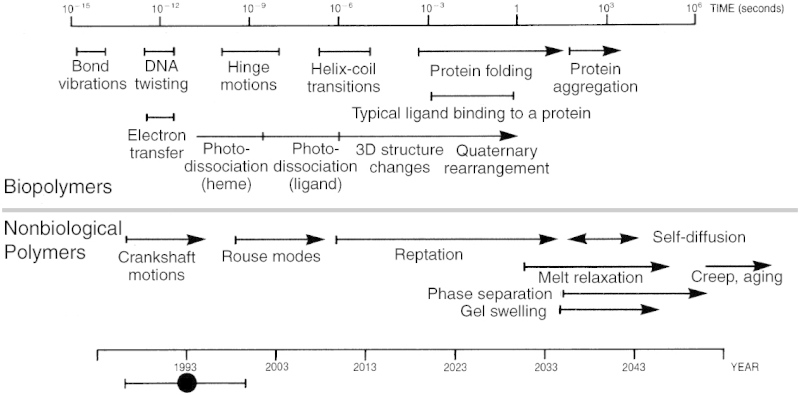
\includegraphics[width=\textwidth]{intro/simulation_timeline.png}
\caption{
Time scales for various motions within biopolymers (upper) and nonbiological
polymers (lower). The year scale at the bottom shows estimates of when each
such process might be accessible to brute force molecular simulation on
supercomputers, assuming that parallel processing capability on supercomputers
increases by about a factor of 1,000 every 10 years (i.e., one order of
magnitude more than Moore's law) and neglecting new approaches or
breakthroughs. Reprinted with permission from H.S. Chan and K. A. Dill.
Physics Today, 46, 2, 24, (1993).
\cite{Chan1993}
    }
\label{fig:intro-timeline}
\end{figure}
%%%%%%%%%%%%%%%%%%%% Simulation Timeline %%%%%%%%%%%%%%%%%%%%%%%%%%%%%%%%%%%



\end{section}


